% !TEX root = ../review.tex
\begin{frame}
\frametitle{OMBlast: Общие сведения}

\end{frame}

\begin{frame}
\frametitle{OMBlast: Алгоритм}

Этапы выравнивания:
\begin{itemize}
  \item Поиск стартовых мест (сидов) для начала выравнивания
  \item Расширение сидов
  \item Объединение пересекающих выравниваний
  \item Построение итогового выравнивания
\end{itemize}

\end{frame}

\begin{frame}
\frametitle{OMBlast: Поиск стартовых сидов - индексация}
  Фрагмент $q$ на карте совпадает с фрагментом $r$ на референсе:
  \begin{equation*}
    r(1 - T_s) - T_m \le q \le r(1 + T_s) + T_m
  \end{equation*}
  $T_s$ - ошибка масштабирования \\
  $T_m$ - ошибка измерений \\
  \begin{figure}
    \centering
    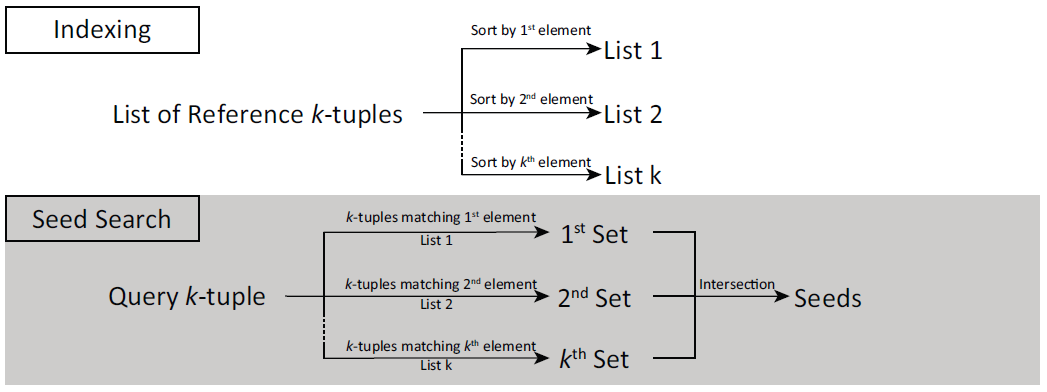
\includegraphics[width = 0.9\textwidth]{omblast/index_A}
  \end{figure}
\end{frame}

\begin{frame}
\frametitle{OMBlast: Поиск стартовых сидов - бины}
  \begin{figure}
    \centering
    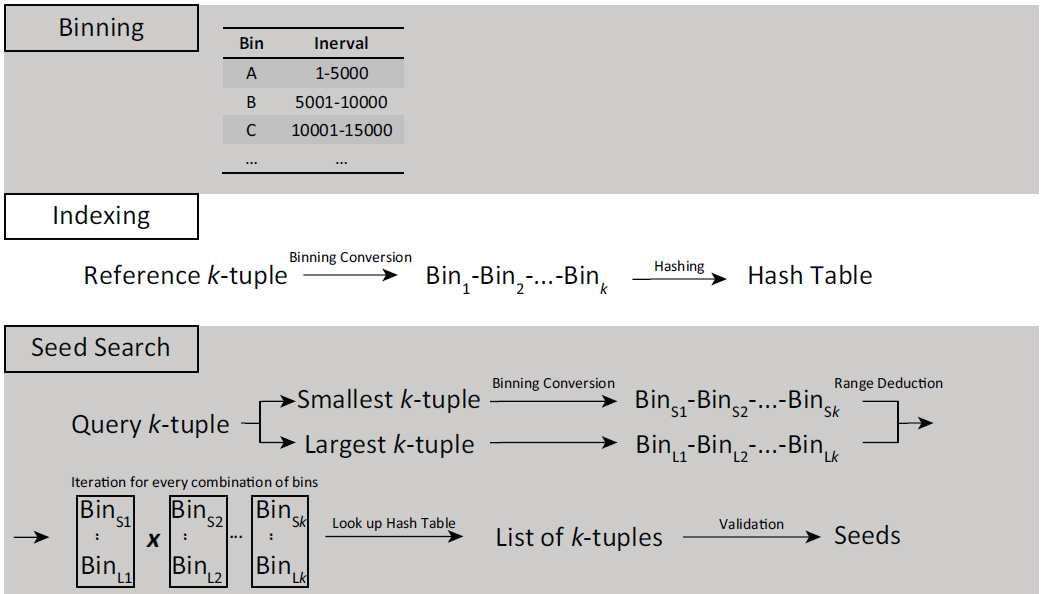
\includegraphics[width = 0.9\textwidth]{omblast/index_B}
  \end{figure}
\end{frame}

\begin{frame}
\frametitle{OMBlast: Расширение сидов}
  \begin{figure}
    \centering
    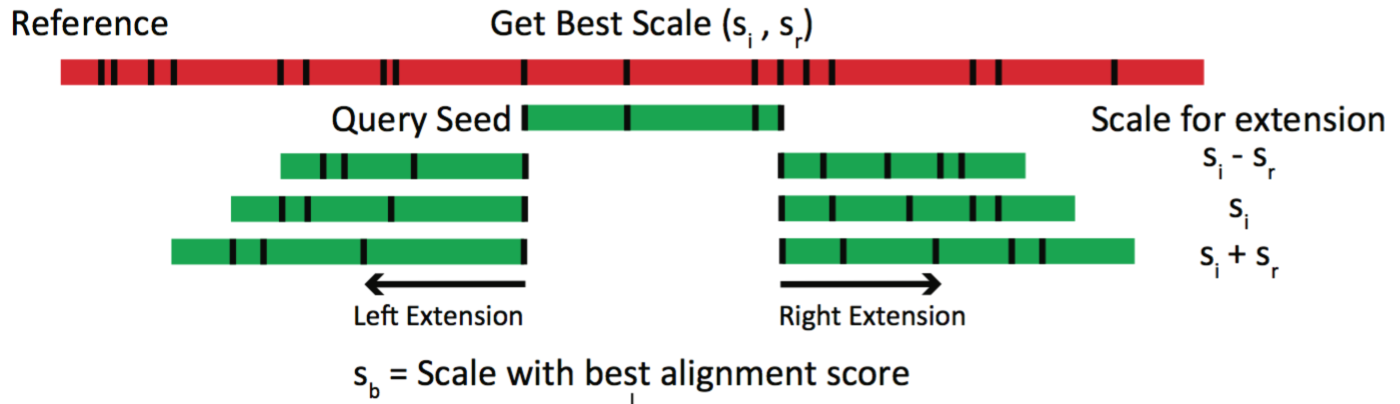
\includegraphics[width = 0.9\textwidth]{omblast/ext_seeds_1}
  \end{figure}
  \begin{figure}
    \centering
    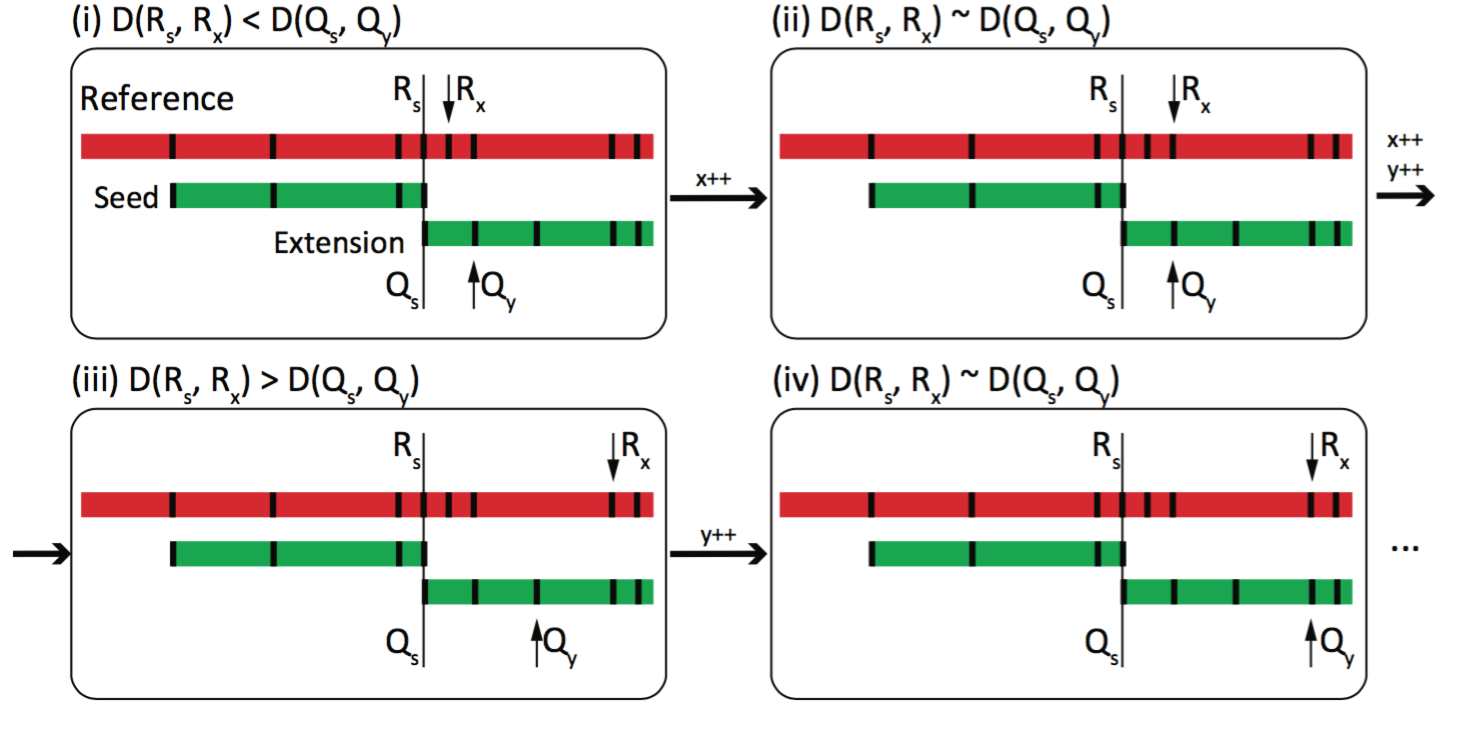
\includegraphics[width = 0.9\textwidth]{omblast/ext_seeds_2}
  \end{figure}
\end{frame}

\begin{frame}
\frametitle{OMBlast: Объединение выравниваний (1)}
  Строится взвешенный ациклический граф:
  \begin{itemize}
    \item Вершины - выравненные разрезы
    \item Рёбра - между двумя парами последовательно (на одной карте) выравненных разрезов
    \item Веса - $t_m \, u_m - t_{es} \, u_{es} - t_{ms} \, u_{ms}$ \\
    $u_{m}$ - количество совпадений\\
    $u_{es}$ - количество лишних разрезов\\
    $u_{ms}$ - количество пропущенных разрезов
  \end{itemize}
  \begin{figure}
    \centering
    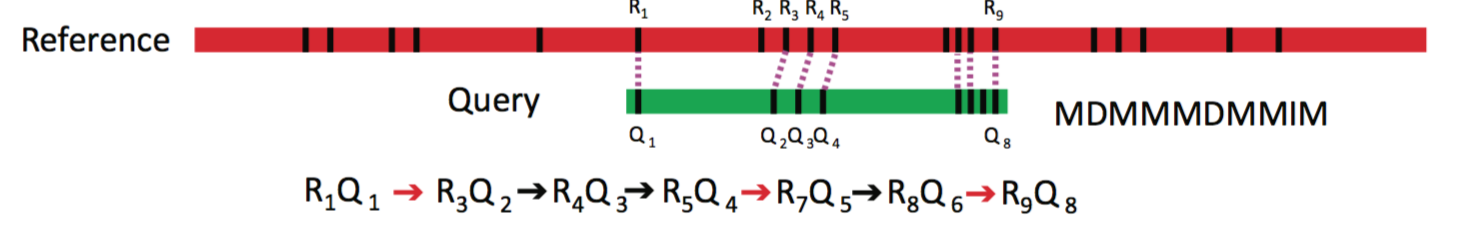
\includegraphics[width = 0.9\textwidth]{omblast/alg_mrg_0}
  \end{figure}
\end{frame}

\begin{frame}
\frametitle{OMBlast: Объединение выравниваний (2)}
  \begin{figure}
    \centering
    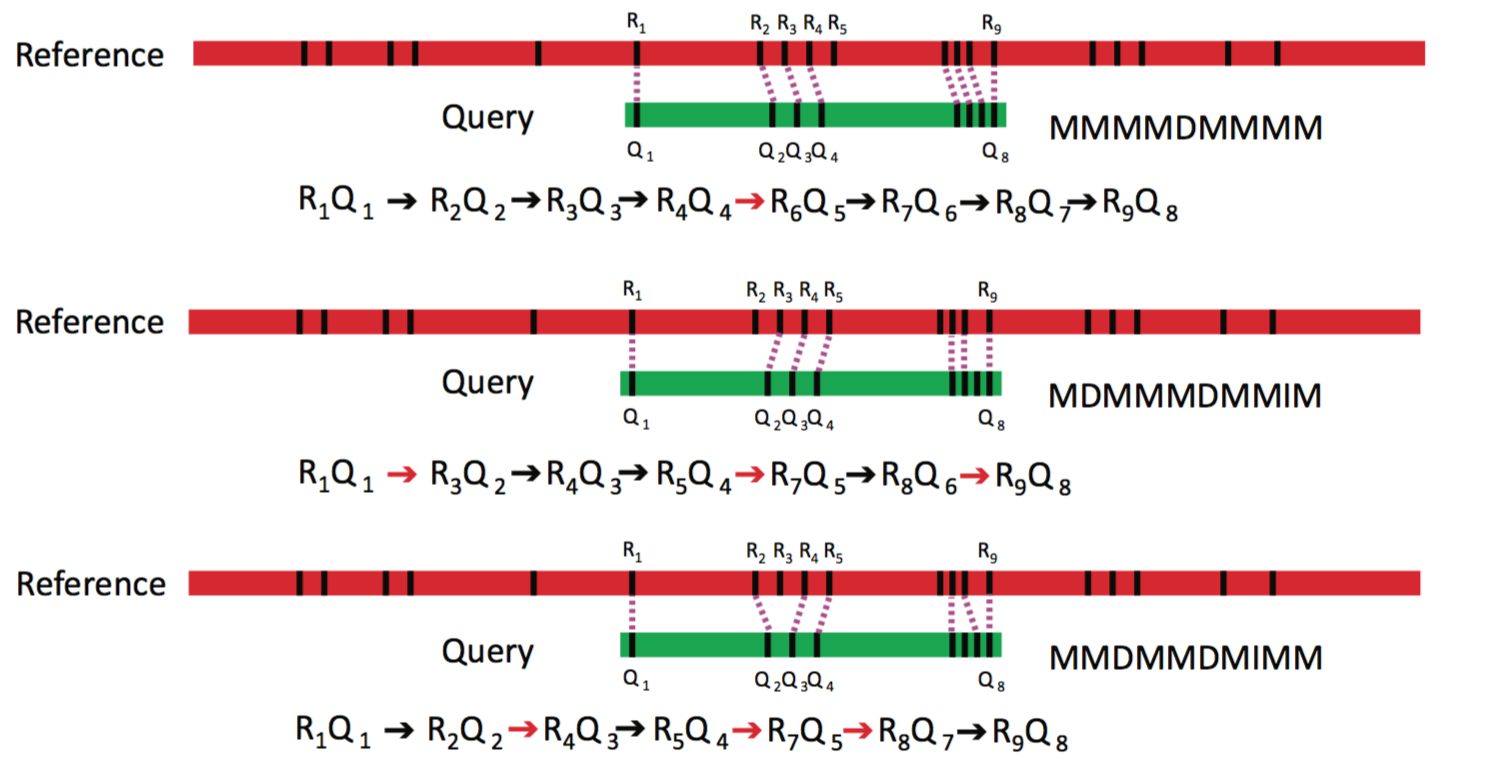
\includegraphics[width = 0.9\textwidth]{omblast/alg_mrg_2}
  \end{figure}
  \begin{figure}
    \centering
    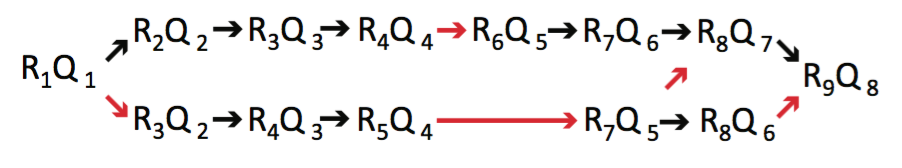
\includegraphics[width = 0.9\textwidth]{omblast/alg_mrg_3}
  \end{figure}

\end{frame}

\begin{frame}
\frametitle{OMBlast: Объединение выравниваний (3)}
С помощью динамического программирования определяется путь в графе с наибольшим весом
  \begin{figure}
    \centering
    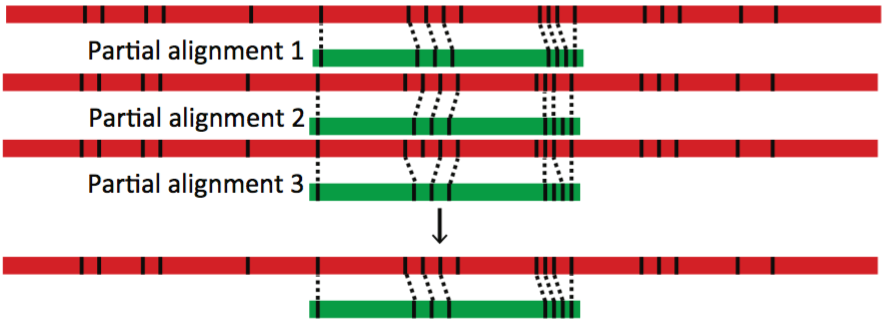
\includegraphics[width = 0.9\textwidth]{omblast/alg_mrg_1}
  \end{figure}

\end{frame}


\begin{frame}
\frametitle{OMBlast: Построение итогового выравнивания}


\end{frame}

\begin{frame}
\frametitle{OMBlast: Результаты - входные данные}
  \begin{figure}
    \centering
    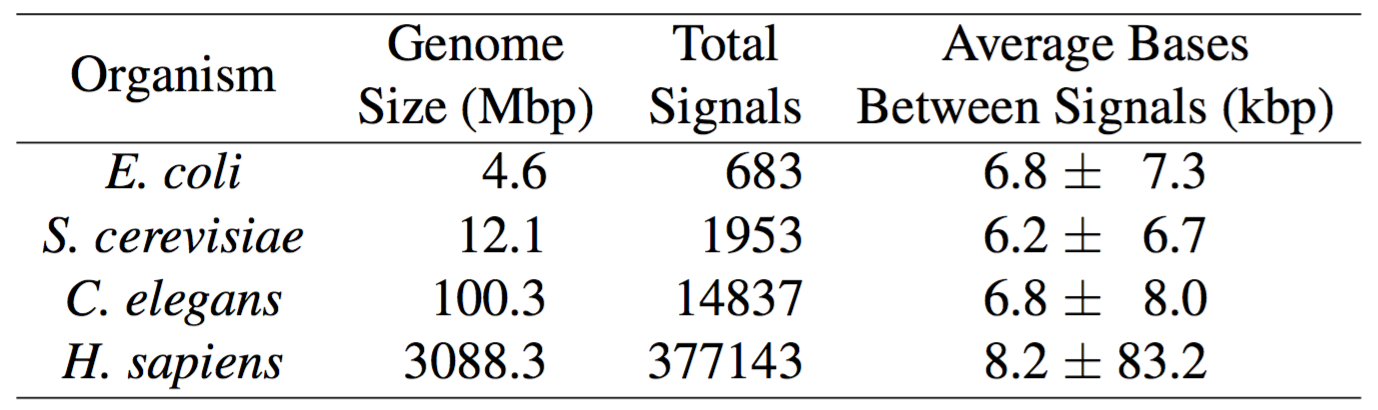
\includegraphics[width = 0.9\textwidth]{omblast/data}
  \end{figure}
  \begin{figure}
    \centering
    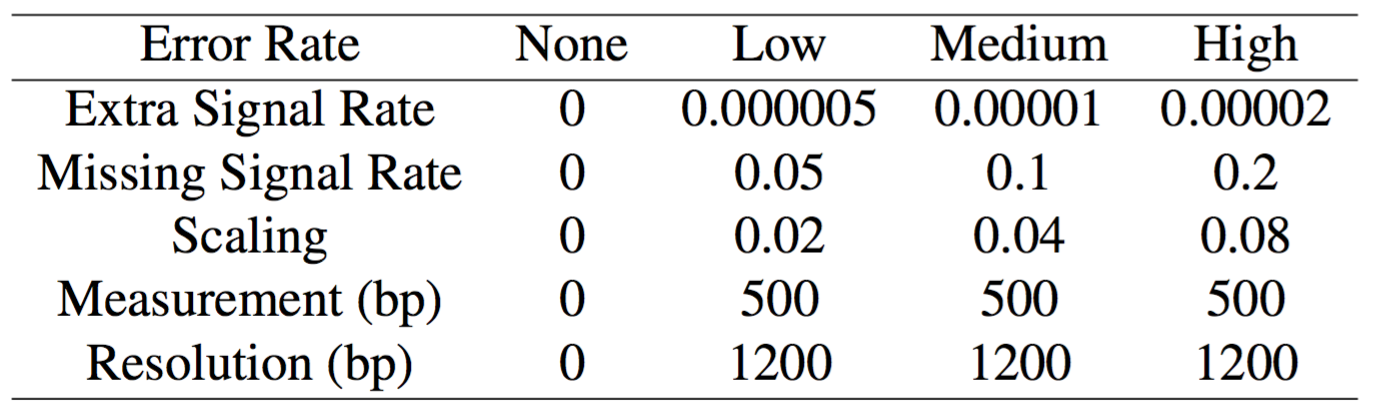
\includegraphics[width = 0.9\textwidth]{omblast/error_levels}
  \end{figure}
\end{frame}

\begin{frame}
\frametitle{OMBlast: Результаты - время работы}
  \begin{figure}
    \centering
    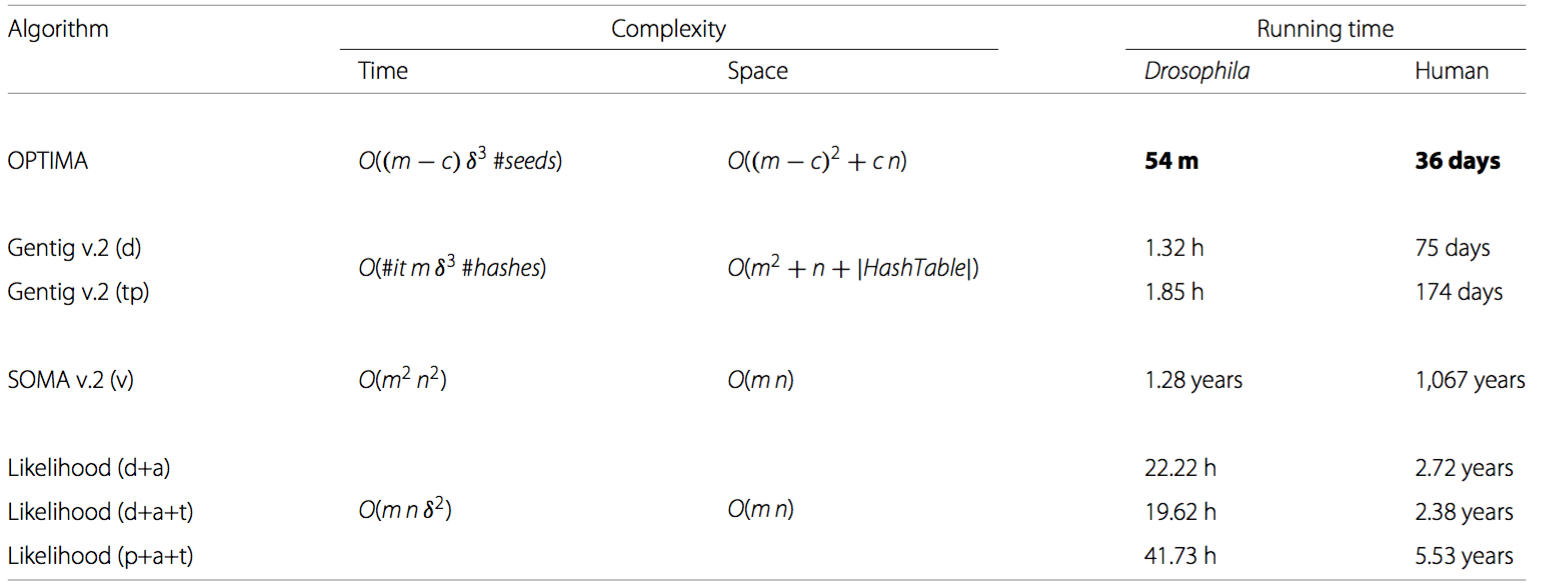
\includegraphics[width = 0.9\textwidth]{omblast/time}
  \end{figure}

\end{frame}

\begin{frame}
\frametitle{OMBlast: Результаты - точность и полнота }
  \begin{figure}
    \centering
    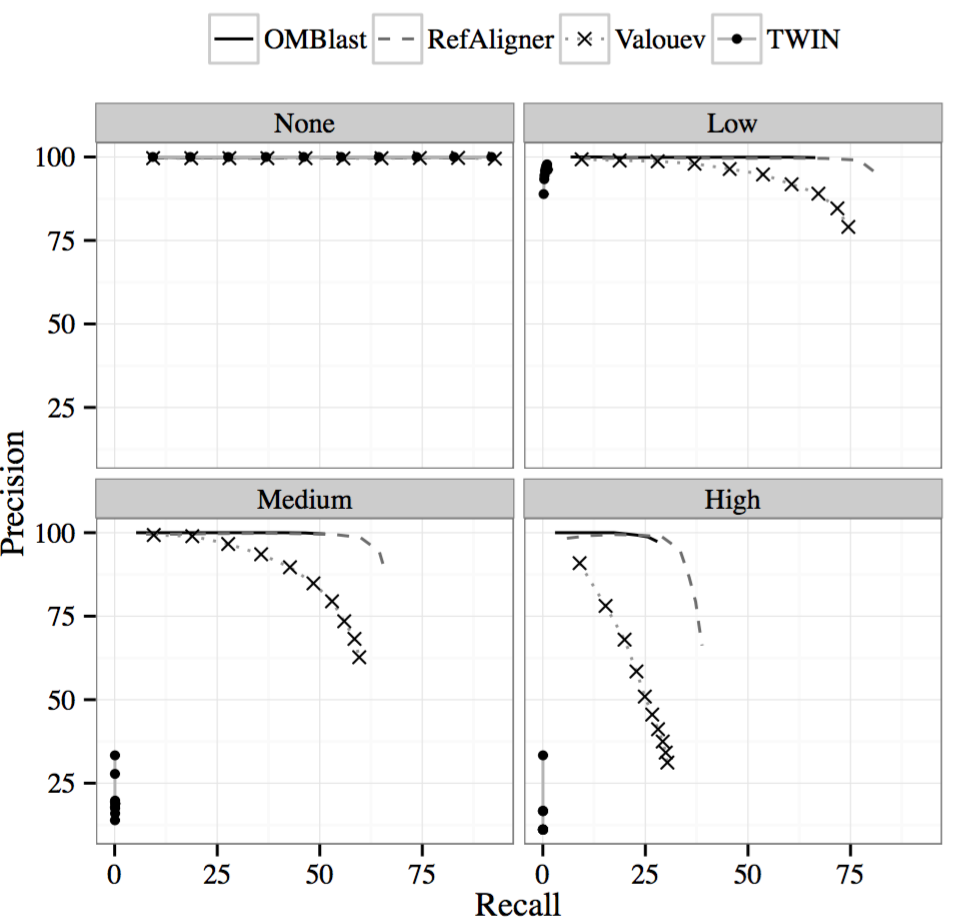
\includegraphics[width = 0.9\textwidth, height = 0.9\textheight]{omblast/error}
  \end{figure}

\end{frame}

\begin{frame}
\frametitle{OMBlast: Результаты - наличие SV}
  \begin{figure}
    \centering
    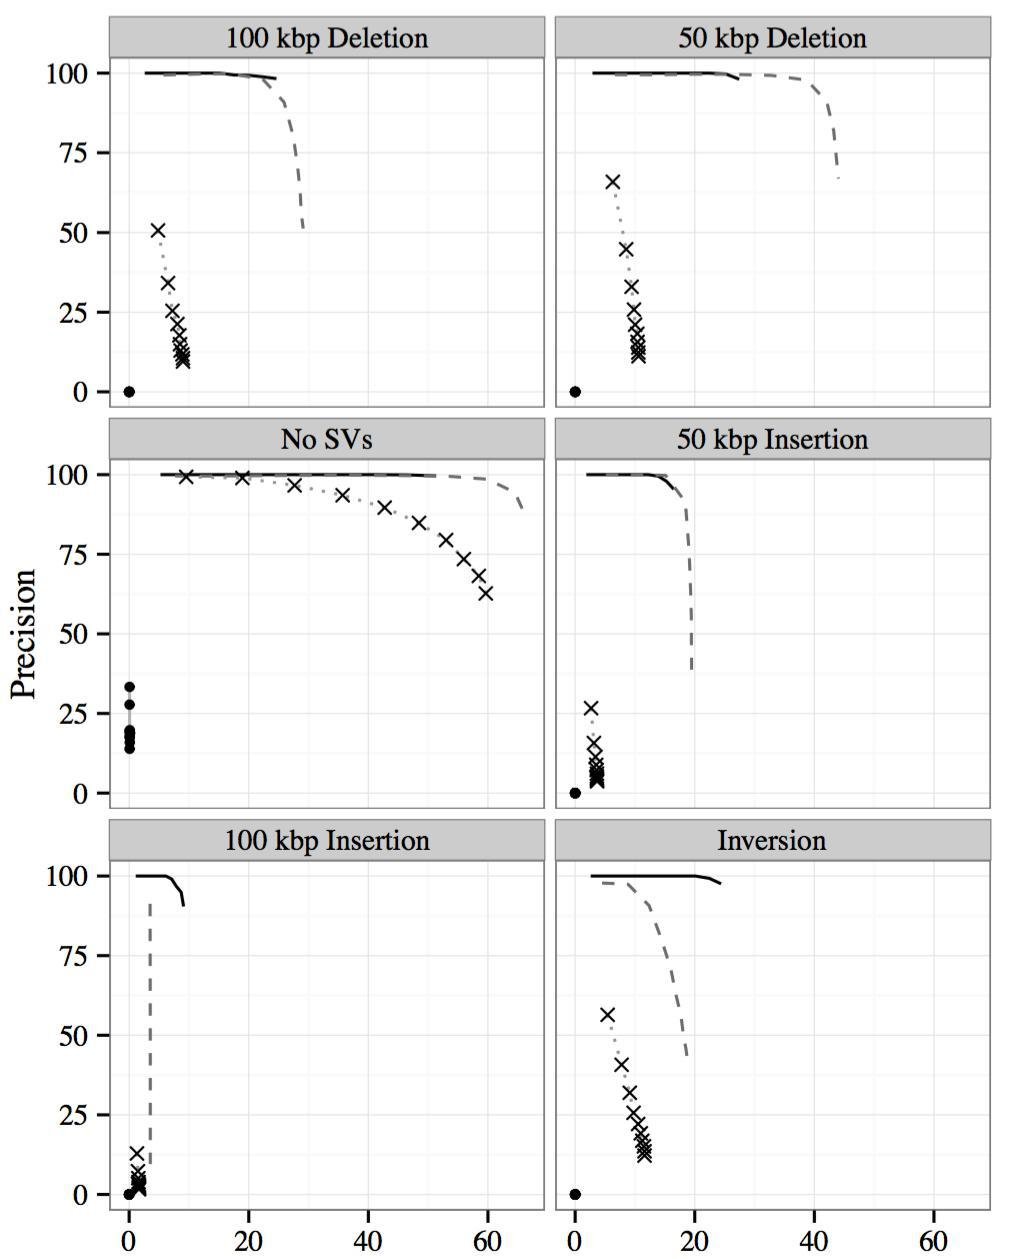
\includegraphics[width = 0.9\textwidth, height = 0.9\textheight]{omblast/sv}
  \end{figure}

\end{frame}
